\subsection{Címsorok}

%18
\begin{frame}
  \begin{itemize}
    \item \texttt{<h1>}, \texttt{<h2>}, \dots, \texttt{<h6>}: legmagasabbtól legalacsonyabb szintig
    \item Például: \texttt{<h1>Első fejezet, amelyben bemutatnak bennünket Micimackónak és a méheknek, mellékesen a könyv is elkezdődik</h1>}
    \item Általában nagyobb betűméretek és a címsor elé és/vagy mögé tett térközök jellemzik
    \item Keresőmotorok is használhatják a dokumentum struktúrájának feltérképezésére
    \item Tematikus részek elválasztására gyakran elválasztó vonalat (\texttt{<hr />}) használnak
  \end{itemize}
\end{frame}

%19
\begin{frame}
  \begin{columns}[c]
    \column{0.5\textwidth}
      Készítsen weboldalt, ami egymás alá írja a \emph{Címsor1}, \emph{Címsor2}, \dots, \emph{Címsor6} szövegeket, a nekik megfelelő HTML elemekkel, a 3. és a 4. szövegsor között pedig húz egy vízszintes vonalat!
    \column{0.5\textwidth}
      \begin{exampleblock}{\textattachfile{cimsorok.html}{cimsorok.html}}
        \begin{center}
          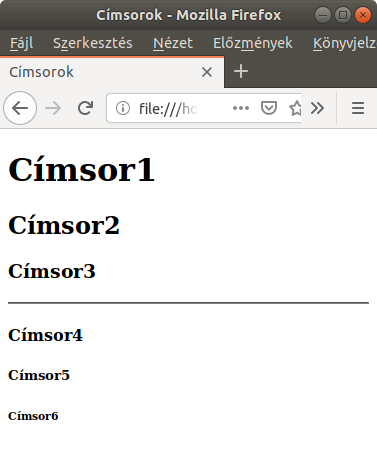
\includegraphics[scale=.25]{cimsorok.png}
        \end{center}
      \end{exampleblock}
  \end{columns}
\end{frame}
